\documentclass[12pt]{article}
\usepackage{times} 			% use Times New Roman

\usepackage[margin=1in]{geometry}   % sets 1 inch margins on all sides
\usepackage[hidelinks]{hyperref}               % for URL formatting
\usepackage[pdftex]{graphicx}       % So includegraphics will work
\setlength{\parskip}{1em}           % skip 1em between paragraphs
\usepackage{indentfirst}            % indent the first line of each paragraph
\usepackage{datetime}
\usepackage[small, bf]{caption}
\usepackage{listings}               % for code listings
\usepackage{xcolor}                 % for styling code
\usepackage{multirow}

%New colors defined below
\definecolor{backcolour}{RGB}{246, 246, 246}   % 0xF6, 0xF6, 0xF6
\definecolor{codegreen}{RGB}{16, 124, 2}       % 0x10, 0x7C, 0x02
\definecolor{codepurple}{RGB}{170, 0, 217}     % 0xAA, 0x00, 0xD9
\definecolor{codered}{RGB}{154, 0, 18}         % 0x9A, 0x00, 0x12

%Code listing style named "gcolabstyle" - matches Google Colab
\lstdefinestyle{gcolabstyle}{
  basicstyle=\ttfamily\small,
  backgroundcolor=\color{backcolour},   
  commentstyle=\itshape\color{codegreen},
  keywordstyle=\color{codepurple},
  stringstyle=\color{codered},
  numberstyle=\ttfamily\footnotesize\color{darkgray}, 
  breakatwhitespace=false,         
  breaklines=true,                 
  captionpos=b,                    
  keepspaces=true,                 
  numbers=left,                    
  numbersep=5pt,                  
  showspaces=false,                
  showstringspaces=false,
  showtabs=false,                  
  tabsize=2
}

\lstset{style=gcolabstyle}      %set gcolabstyle code listing

% to make long URIs break nicely
\makeatletter
\g@addto@macro{\UrlBreaks}{\UrlOrds}
\makeatother

% for fancy page headings
\usepackage{fancyhdr}
\setlength{\headheight}{13.6pt} % to remove fancyhdr warning
\pagestyle{fancy}
\fancyhf{}
\rhead{\small \thepage}
\lhead{\small HW0, Maynard} 
\chead{\small DATA 440, Fall 2024} 

%-------------------------------------------------------------------------
\begin{document}

% EDIT THE ITEMS HERE
\begin{centering}
{\large\textbf{HW0 - Getting Started with Assignment reports and Linux command-line utilities}}\\ 
Courtney Maynard\\
September 8th, 2024(September 10th, 2024)\\
\end{centering}

%-------------------------------------------------------------------------

% The * after \section just says to not number the sections
\section*{Q3}

\emph{Replace the "Growth of the Early Web" image. Make sure to change the image caption and description of the image in the report, too.}

\subsection*{Answer}

Figure \ref{fig:courtney-hiking} shows me hiking in Acadia National Park this past summer.

\begin{figure}[h]
    \centering
    % trim and clip are used to crop the image, trim=left bottom right top
    % width sets max width, height will be scaled appropriately
    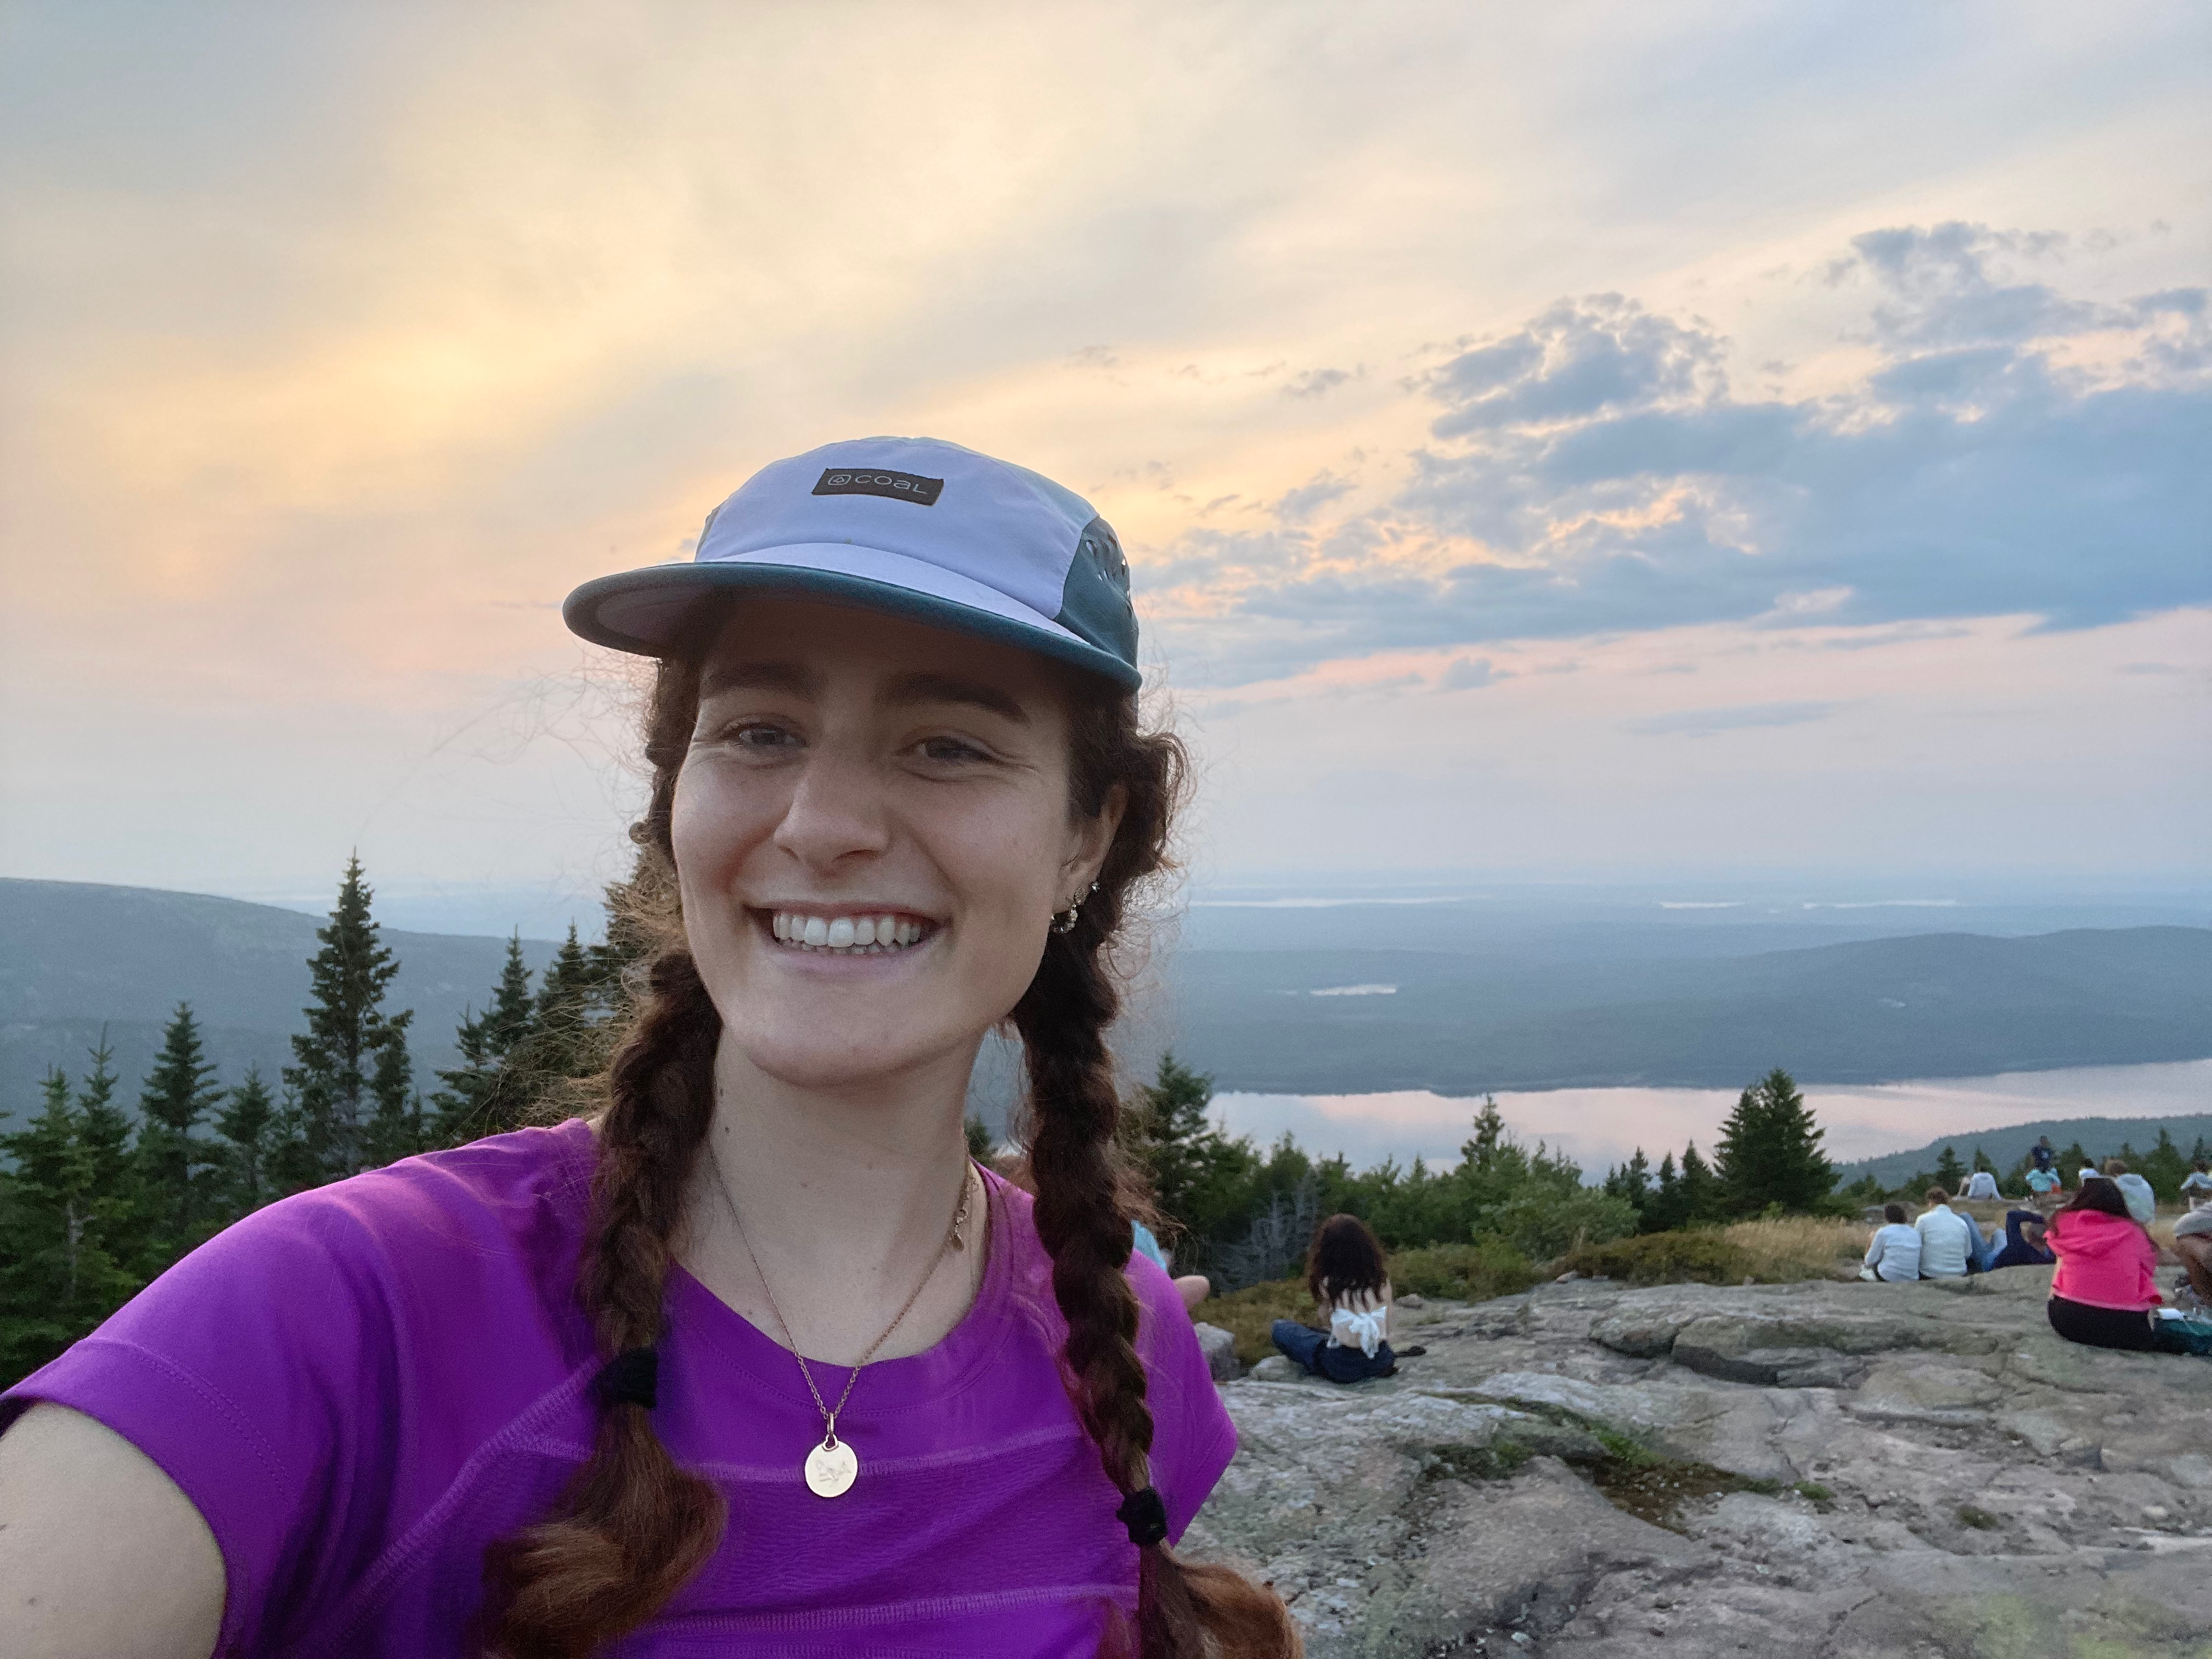
\includegraphics[trim=0 20 10 50, clip, width=\textwidth]{hiking.png}
    \caption{Courtney hiking in Acadia National Park}
    \label{fig:courtney-hiking}
\end{figure}

\subsection*{Discussion}

I arrived at the image shown above by following the template for uploading an image in Latex. The implication of this exercise is that I now know how to display images in Latex.

\section*{Q4}

\emph{Replace the code in the lstlisting environment with another block of code. You can use some Python code, or you can insert code from a different language -- just change the language indicated so that syntax highlighting still works properly. Make sure to change the caption as needed.}

\subsection*{Answer}

Listing \ref{lst:copy} is an example of directly copying code into the LaTeX document and having the listings package perform syntax highlighting. Listing \ref{lst:import} is an example of importing the code from a file rather than copying it in.

%Python code highlighting
\begin{lstlisting}[language=Python, caption=Tokenization of song lyrics copied into the LaTeX, label=lst:copy]
# must split lyrics into lines, in order to retain the line-level information.
def lyrics_into_lines(lyrics):
    return lyrics.split('\n')

df_balanced['Lyrics_Lines'] = df_balanced['Lyrics'].apply(lyrics_into_lines)

# tokenize each line individually in order to respect the structure of the song.

def tokenize_line(line):
    line = re.sub(r'[^a-zA-Z0-9\s]', '', line.lower())
    tokens = word_tokenize(line)
    return tokens

def tokenize_lyrics(lines):
    return [tokenize_line(line) for line in lines]

df_balanced['Tokenized_Lyrics'] = df_balanced['Lyrics_Lines'].apply(tokenize_lyrics)
\end{lstlisting}

%Importing code from file
\lstinputlisting[language=Python, caption=Tokenization of song lyrics loaded from file, label=lst:import]{websciencehwzeroexample.py}

\subsection*{Discussion}

I followed the template to figure out how to display python code in the two different ways: through directly pasting it in and through uploading a file. As a result of this exercise, I now know how to display code in Latex using two different methods.

\section*{Q5}

\emph{Edit Table 1 so that it matches the first 4 weeks of our class schedule, as given in our syllabus.}

\subsection*{Answer}

Table \ref{tbl:schedule} shows our class syllabus for the first four weeks.

\begin{table}[h]
\centering
\caption{First Four Weeks Schedule}
\label{tbl:schedule}
\begin{tabular}{|l|l|p{50mm}|p{70mm}|}
\hline
\textbf{Week} & \textbf{Lecture Dates} & \textbf{Topic} & \textbf{Homework (Date Assigned -- Due Date} \\ \hline \hline
01 & Aug 29 \& Sep 3 & \href{https://docs.google.com/presentation/d/1sSNcXMBUJWb-rVbTEvKqFAC2SvJugI8m/edit#slide=id.p1}{Introduction to Web Science and Web Architecture} & \href{https://github.com/anwala/teaching-web-science/tree/main/fall-2024/homework/hw0}{HW0} - Getting started, Aug 29 - - Sep 10 \\ \hline
02 & Sep 5 \& 10 & \href{https://docs.google.com/presentation/d/1_TcgFerDRT0dZVX98-jMIJBMmV4_IAQg/}{Introduction to Python} & \href{https://github.com/anwala/teaching-web-science/blob/main/fall-2022/week-2/data_440_03_f22_mod_02_python.ipynb}{Python Google Colab notebook} \newline \href{https://github.com/anwala/teaching-web-science/blob/main/fall-2022/week-2/data_440_03_f22_mod_02_lab.ipynb}{Python lab exercises} \newline \href{https://github.com/anwala/teaching-web-science/tree/main/fall-2024/homework/hw1}{HW1} - Web Sci. Intro, Sep 10 -- 24 \\ \hline
03 & Sep 12 \& 17 & \href{https://docs.google.com/presentation/d/1pSywHD9i3aVNsWNxtcUfT1E2tP4mgcQv/}{Introduction to Info Vis with R, Python} \newline \href{https://docs.google.com/presentation/d/1vtT9dleNJlUbc3ny14gotGX1Md1dEWhVHYWTz0MMdRk/edit?usp=sharing}{Web Scraping} & \href{https://github.com/anwala/teaching-web-science/blob/main/fall-2022/week-3/data_440_03_f22_mod_03_info_vis_r.ipynb}{InfoVis in R Colab notebook} \newline \href{https://github.com/anwala/teaching-web-science/blob/main/fall-2022/week-3/data_440_03_f22_mod_03_info_vis_python.ipynb}{InfoVis in Python Colab notebook} \newline \href{https://github.com/anwala/teaching-web-science/blob/main/fall-2023/week-3/data_440_02_f23_mod_03_web_scraping_imdb.ipynb}{Web Scraping (IMDB) Python Colab notebook} \newline \href{https://github.com/anwala/teaching-web-science/blob/main/fall-2023/week-3/twitter-scraper/}{Web Scraping (Twitter) Python scripts} \\ \hline
04 & Sep 19 \& 24 & \href{https://docs.google.com/presentation/d/1R7CKhxlAv_nQtt_xb1HQotqgSxcVDz58/}{Measuring the Web}  &  \\ \hline
\end{tabular}
\end{table}

\subsection*{Discussion}

I used the example table to begin creating this table. In order to make sure that the different homework links were able to be stacked inside their respective columns, I looked at Stackexchange to learn how to format the table correctly. Thus, I changed the column types in order to use the newline command to create the corresponding table. Additionally, I linked all of the respective lectures and homework using the href command, which I knew how to do because of previous Latex experience. Because of this exercise, I now know how to format various types of tables in Latex.

\section*{References}

\begin{itemize}
    \item {Stackexchange - Latex - Table with multiple lines in some cells, \url{https://tex.stackexchange.com/questions/40561/table-with-multiple-lines-in-some-cells}}
    \item {Scribbr - Poisson Distributions | Definition, Formula \& Examples, \url{https://www.scribbr.com/statistics/poisson-distribution/}}
    \item {Computer Science Wiki - Graph theory and connectivity of the web, \url{https://computersciencewiki.org/index.php/Graph_theory_and_connectivity_of_the_web}}
\end{itemize}

\end{document}

